\documentclass[aspectratio=169]{beamer}

\usepackage[utf8]{inputenc}
\usepackage{tikz}
\usepackage[absolute, overlay]{textpos}
\usepackage{media9}
\usepackage{tabularx}
\usepackage{pifont}
\usepackage{smartdiagram}
\usepackage{pgf-umlsd}
\usepackage{listings}
\usepackage{booktabs}
\usepackage{multicol}

\usetikzlibrary{positioning}

\title{DriveBuild}
\subtitle{Interactive session and demonstration}
\author{Stefan Huber}
\institute{University of Passau}
\date{\today}

\usetheme{Rochester}
\beamertemplatenavigationsymbolsempty%

\newcommand{\draft}[1]{\color{red} \itshape{} #1}
\newcommand{\includeFSVideo}[1]{%
    \begin{textblock*}{5pt} (0pt, 0pt)
        \includemedia[
            height=\paperheight,
            width=\paperwidth,
            addresource=#1,
            activate=pageopen,
            playbutton=none,
            passcontext,
            flashvars={source=#1&autoPlay=true&loop=true}
        ]{}{VPlayer9.swf}
    \end{textblock*}
}

\newcommand{\videoframe}[1]{%
    \begin{frame}[plain]
        \includeFSVideo{#1}
    \end{frame}
}

\AtBeginSection[]{%
    \begin{frame}
    \vfill
    \centering
    \begin{beamercolorbox}[sep=8pt,center,shadow=true,rounded=true]{title}
        \usebeamerfont{title}\insertsectionhead\par%
    \end{beamercolorbox}
    \vfill
    \end{frame}
}

\begin{document}

\maketitle%

\begin{frame}{Overview}
    \tableofcontents%
\end{frame}

\section{Components of a Test}
\begin{frame}[plain]
    \begin{textblock*}{\paperwidth} (0pt,0pt)
        \includegraphics[width=\paperwidth]{media/smallGridPlain.png}
    \end{textblock*}
\end{frame}
\subsection{Environment}
\begin{frame}{Lanes}
    \centering
    Lanes = Positions + widths
    \begin{tikzpicture}
        \node (l1) {\includegraphics[width=.8\paperwidth]{media/lanes.png}};
        \pause%
        \node (l2) {\includegraphics[width=.85\paperwidth]{media/2019-05-31_simpleLane.png}};
    \end{tikzpicture}
\end{frame}

\begin{frame}{Obstacles}
    \centering
    \begin{tikzpicture}
        \pause%
        \node (cube) {\includegraphics[height=.7\paperheight]{media/cube.png}};
        \pause%
        \node (cylinder) {\includegraphics[height=.75\paperheight]{media/cylinder.png}};
        \pause%
        \node (bump) {\includegraphics[width=\linewidth]{media/bump.png}};
        \pause%
        \node (cone) {\includegraphics[height=.8\paperheight]{media/cone.png}};
        \pause%
        \node (obstacles) {\includegraphics[height=.8\paperheight]{media/obstacles.png}};
    \end{tikzpicture}
\end{frame}

\begin{frame}[plain]
    \centering
    \Huge Questions so far?
\end{frame}

\begin{frame}{What about these?}
    \begin{itemize}[<+(1)->] % chktex 36
        \item Can I model hills?
        \item Any chance to model ``ramps''?
        \item How does the rotation work?
        \item Can I change the lane material?
        \item What about the weather and the time of day?
        \item Have lanes additional information like direction or position on the lane?
    \end{itemize}
\end{frame}

\subsection{Participants}
\begin{frame}{Description of Participants}
    \centering
    \begin{tikzpicture}
        \pause%
        \node (all) {\includegraphics[height=.8\paperheight]{media/models.png}};
        \pause%
        \node (one) {\includegraphics[height=.8\paperheight]{media/models_onlyETK800.png}};
    \end{tikzpicture}
\end{frame}

\begin{frame}{Description of Participants}
    \centering
    \begin{tikzpicture}
        \node (car) {\includegraphics[height=.75\paperheight]{media/carFromTop.png}};
        \pause%
        \onslide<2>\node (position) at (4,0) {\includegraphics[height=.3\paperheight]{media/position.png}};
        \pause%
        \node (rotation) {\includegraphics[height=.8\paperheight]{media/rotation.png}};
    \end{tikzpicture}
\end{frame}

\begin{frame}{Description of Movements}
    \centering
    \includegraphics[width=\linewidth]{media/waypoints.png}
\end{frame}

\begin{frame}{Waypoint}
    \centering
    \begin{tikzpicture}
        \node (waypoint) at (0,0) {\includegraphics[height=.8\paperheight]{media/waypoint.png}};
        \pause%
        \node (position) at (6,0) {\includegraphics[width=.2\paperwidth]{media/position.png}};
        \pause%
        \coordinate (a) at (0,0.1);
        \coordinate (b) at (3.2,0.1);
        \draw[<->, red, ultra thick] (a) -- (b) node[midway, above]{tolerance};
    \end{tikzpicture}
\end{frame}

\begin{frame}{Movement Modes}
    \setlength{\columnsep}{-6cm}
    \begin{multicols}{2}
        \begin{itemize}[<+(1)->] % chktex 36
            \item MANUAL
            \item AUTONOMOUS
            \item TRAINING
        \end{itemize}
        \pause%
        \includegraphics[width=\linewidth]{media/2019-06-05_ParticipantMovement.png} % chktex 8
    \end{multicols}
\end{frame}

\begin{frame}{MANUAL Mode Feature}
    \begin{multicols}{2}
        \pause%
        \includegraphics[width=\linewidth]{media/minSpeed.png}
        \pause%
        \includegraphics[height=.7\paperheight]{media/speedLimit.png}
    \end{multicols}
\end{frame}

\subsection{AIs}
\begin{frame}[plain]
    \centering
    \resizebox{!}{.95\paperheight}{%
        \begin{sequencediagram}
            \newthread{user}{User}{}
            \newinst{ai}{:AI}{}
            \newthread{sim}{:Simulation}{}
            \begin{callself}{sim}{\(simulate()\)}{}
                \postlevel\postlevel%
                \postlevel\postlevel%
            \end{callself}

            \prelevel\prelevel%
            \prelevel\prelevel%
            \prelevel%
            \begin{call}{user}{\(start()\)}{ai}{}
                \begin{sdblock}{Repeat}{}
                    \begin{call}{ai}{\(wait()\)}{sim}{ready}
                    \end{call}
                    \begin{call}{ai}{\(request()\)}{sim}{data}
                    \end{call}
                    \begin{call}{ai}{\(control()\)}{sim}{}
                    \end{call}
                \end{sdblock}
            \end{call}
        \end{sequencediagram}
    }
\end{frame}

\begin{frame}{Available Information}
    \begin{textblock*}{.25\paperwidth} (.6\paperwidth,.2\paperheight)
        \onslide<3-6>{\includegraphics[width=\linewidth]{media/2019-05-31_cameras.png}} % chktex 8
    \end{textblock*}
    \begin{itemize}[<+(1)->] % chktex 36
        \item Sensor data
            \begin{itemize}
                \item Camera (front, back, left, right, dash)
                    \begin{itemize}
                        \item colored
                        \item annotated
                        \item depth
                    \end{itemize}
                \item Speed
                \item Damage
                \item LiDAR
            \end{itemize}
        \item Additional data
            \begin{itemize}
                \item Position
                \item Steering angle
            \end{itemize}
    \end{itemize}
\end{frame}

\videoframe{media/2019-05-31_front_camera_view.mp4} % chktex 8

\begin{frame}{Python Client}
    \centering
    \includegraphics[height=.7\paperheight]{media/python.jpg}
\end{frame}

\begin{frame}[plain]
    \centering
    \Huge Still no questions?
\end{frame}

\begin{frame}{What about these?}
    \begin{itemize}[<+(1)->] % chktex 36
        \item What do I have to do to implement an AI? % chktex 13
        \item Do I need to \(wait()\)?
        \item Do I have to use Python?
        \item How does the TRAINING mode work?
        \item Can I ``fake'' an AI or try out a test without an actual AI? % chktex 13
        \item Do I need an AI when doing TRAINING?
        \item Can I use the built-in AI of BeamNG?
        \item Does the MANUAL mode recognize the tolerance of waypoints?
        \item Can I control things like the gear or the parking brake?
    \end{itemize}
\end{frame}

\subsection{Criteria}
\begin{frame}{Types of planned Criteria}
    \centering
    \begin{tabularx}{.4\linewidth}{X c c}
        \toprule
        \bfseries Type & \bfseries VC & \bfseries SC \\
        \midrule
        position       & \checkmark{} & \checkmark{} \\
        area           & \checkmark{} & \checkmark{} \\
        lane           & \checkmark{} & \checkmark{} \\
        speed          & \checkmark{} & \checkmark{} \\
        damage         & \checkmark{} & \checkmark{} \\
        time           & \checkmark{} & \ding{53}    \\
        distance       & \checkmark{} & \checkmark{} \\
        TTC            & \checkmark{} & \ding{53}    \\
        light          & \checkmark{} & \checkmark{} \\
        waypoint       & \checkmark{} & \checkmark{} \\
        \bottomrule
    \end{tabularx}
\end{frame}

\begin{frame}{Description of Criteria}
    \begin{textblock*}{4.7cm} (5mm, 1.7cm)
        \onslide<2->{\includegraphics[width=\linewidth]{media/durchdrehen.jpg}}
    \end{textblock*}
    \centering
    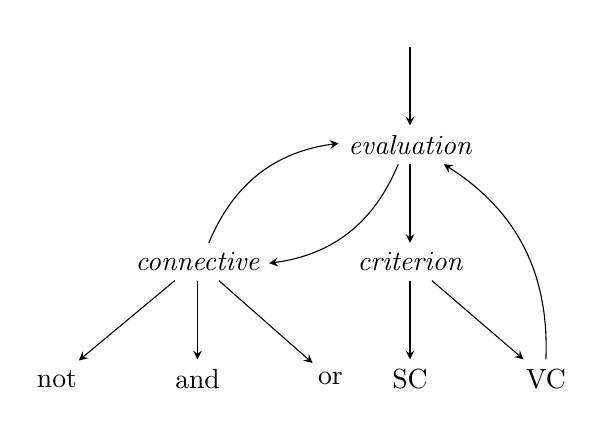
\begin{tikzpicture}[%
        ->,
        >=stealth
    ]
        \node (evaluation) {\itshape evaluation};
        \node[above=of evaluation] (start) {};
        \node[below=of evaluation] (criterion) {\itshape criterion};
        \node[left=of criterion] (connective) {\itshape connective};
        \node[below=of connective] (and) {and};
        \node[right=of and] (or) {or};
        \node[left=of and] (not) {not};
        \node[below=of criterion] (sc) {SC};
        \node[right=of sc] (vc) {VC};

        \path
            (start) edge (evaluation)
            (evaluation) edge (criterion)
            (evaluation) edge[bend left]  (connective)
            (connective) edge[bend left] (evaluation)
            (criterion) edge (sc)
            (criterion) edge (vc)
            (vc) edge[bend right] (evaluation)
            (connective) edge (not)
            (connective) edge (and)
            (connective) edge (or);
    \end{tikzpicture}
\end{frame}

\begin{frame}{Example}
    \centering
    \includegraphics[width=\linewidth]{media/2019-05-31_simpleLaneWithCriteria.png} % chktex 8
\end{frame}

\videoframe{media/2019-06-08_manualDrive.mp4} % chktex 8

\videoframe{media/2019-06-09_manualDrive_failure.mp4} % chktex 8

\begin{frame}{Example with VCs}
    Speed limit on a certain lane
\end{frame}

\begin{frame}{Criteria on Client Side}
    \centering
    \begin{sequencediagram}
        \newthread{sim}{:Simulation}
        \newinst{ai}{:AI}
        \begin{call}{sim}{\itshape{} data}{ai}{\itshape{} control}
            \begin{call}{ai}{\itshape{} check criteria}{ai}{}
            \end{call}
            \begin{call}{ai}{\itshape{} do calculations}{ai}{}
            \end{call}
            \begin{call}{ai}{\itshape{} check more criteria}{ai}{}
            \end{call}
        \end{call}
    \end{sequencediagram}
\end{frame}

\begin{frame}[plain]
    \centering
    \Huge Really? No questions?
\end{frame}

\begin{frame}{What about these?}
    \begin{itemize}[<+(1)->] % chktex 36
        \item Why is there a speed criterion if there are already a target speed as well as a speed limit in the MANUAL mode?
        \item Which of the planned criteria do you need?
        \item Do you need any further criteria?
        \item Do you need additional information during simulation?
    \end{itemize}
\end{frame}

\section{Execution of Tests}
\begin{frame}{Runtime verification/Synchronous Simulation}
    \centering
    \smartdiagram[circular diagram:clockwise]{%
        Verify criteria, Request AIs, Control, Start Resume, Pause
    }
\end{frame}

\begin{frame}{Checking Criteria}
    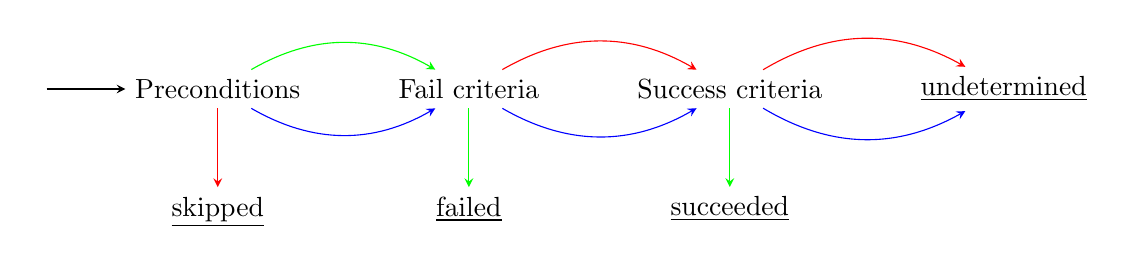
\begin{tikzpicture}[%
        ->,
        >=stealth
    ]
        \node (start) {};
        \node[right=of start] (preconds) {Preconditions};
        \node[below=of preconds] (skipped) {\underline{skipped}};
        \node[right=of preconds] (fail) {Fail criteria};
        \node[below=of fail] (tcFail) {\underline{failed}};
        \node[right=of fail] (success) {Success criteria};
        \node[below=of success] (tcSuccess) {\underline{succeeded}};
        \node[right=of success] (undetermined) {\underline{undetermined}};

        \path (start) edge (preconds);
        \draw[red] (preconds) edge (skipped);
        \draw[green] (preconds) edge[bend left] (fail);
        \draw[blue] (preconds) edge[bend right] (fail);
        \draw[green] (fail) edge (tcFail);
        \draw[red] (fail) edge[bend left] (success);
        \draw[blue] (fail) edge[bend right] (success);
        \draw[green] (success) edge (tcSuccess);
        \draw[red] (success) edge[bend left] (undetermined);
        \draw[blue] (success) edge[bend right] (undetermined);
    \end{tikzpicture}
\end{frame}

\begin{frame}{GUI}
    A ``GUI'' is missing so far\ldots\\
    \pause%
    And it may never come\ldots\\
    \pause%
    Currently stick to HTTP GET requests, i.\,e.\ the provided client
\end{frame}

\section{How to use it?}
\begin{frame}{Test Generation}
    Goal: Generate XML files\\
    Therefore:
    \begin{enumerate}[<+(1)->] % chktex 36
        \item Implement the methods and strategies of your paper
        \item Implement a converter translating the output to DriveBuild files
        \item Test generated files
    \end{enumerate}
\end{frame}

\begin{frame}{Training AIs}
    Goal: Collect training data for AIs (e.\,g.\ neural networks)\\
    Therefore:
    \begin{enumerate}[<+(1)->] % chktex 36
        \item Think about the data you need
        \item Think about an scenario presumably delivering that data
            \begin{itemize}
                \item Lanes
                \item Obstacles
                \item Participants
                \item Movements (E.\,g.\ do participants meet?)
            \end{itemize}
        \item Train an AI
        \item Test trained AI
    \end{enumerate}
\end{frame}

\begin{frame}[plain]
    \centering
    \Huge Any other application {\bfseries you} want me to explain or to think about?
\end{frame}

\begin{frame}[plain]
    \centering
    \Huge Last chance for questions!\\
    \huge Use it!
\end{frame}

\end{document}
